\documentclass{article}
\usepackage[T1]{fontenc}
\usepackage[utf8]{inputenc}
\usepackage[a4paper, total={6in, 11in}]{geometry}
\usepackage{algorithm}
\usepackage{amsfonts}
\usepackage{algpseudocode}
\usepackage{float}
\usepackage{graphicx}
\usepackage{subcaption}
\usepackage{amsmath}

\title{%
	Obliczenia naukowe \\
	\large Lista 5}
\author{Szymon Janiak}
\begin{document}
\maketitle

\section*{Opis problemu}
	Głównym problemem jest rozwiązanie równania liniowego\\
	\centerline{$Ax = b$},
	gdzie macierz A jest rzadką, tj. mającą dużą elementów zerowych, i blokową o następującej strukturze:\\
	\[
	A = \begin{bmatrix}
	A_1 & C_1 & 0 & 0 & \dots & 0 \\
	B_2 & A_2 & C_2 & 0 & \dots & 0 \\
	0 & B_3 & A_3 & C_3 & \dots & 0 \\
	\vdots & \vdots & \vdots & \ddots & \vdots \\
	0 & \dots & 0 & B_{v-2} & A_{v-2} & C_{v-2} \\
	0 & \dots & 0 & 0 & B_{v-1} & A_{v-1} \\
	0 & \dots & 0 & 0 & 0 & B_v A_v \\
	\end{bmatrix}
	\]
	i wektora prawych stron $\mathbf{b} \in \mathbb{R}^{n \times n}$, gdzie $n \geq 4$.\\
	\\
	Niech $v = \frac{n}{\ell}$, zakładając, że $n$ jest podzielne przez $\ell$, gdzie $\ell$ jest rozmiarem wszystkich kwadratowych macierzy wewnętrznych (bloków): $A_k$, $B_k$ i $C_k$. Mianowicie, $A_k \in \mathbb{R}^{\ell \times \ell}$, dla $k = 1, \ldots, v$ jest macierzą gęstą, $0$ jest kwadratową macierzą zerową stopnia $\ell$, a macierz $B_k \in \mathbb{R}^{\ell \times \ell}$, dla $k = 2, \ldots, v$ ma następującą postać:\\
	\[
	B_k = \begin{bmatrix}
	    0 & \dots & 0 & b_{k1} \\
	    0 & \dots & 0 & b_{k2} \\
	    \vdots & \vdots & \vdots & \vdots \\
	    0 & \dots & 0 & b_{k\ell}
	\end{bmatrix}
	\]\\

	Macierz $B_k$ ma tylko jedną, ostatnią, kolumnę niezerową. Natomiast $C_k \in \mathbb{R}^{\ell \times \ell}$, dla $k = 1, \ldots, v - 1$, jest macierzą diagonalną:\\
	\[
	C_k = \begin{bmatrix}
	    c_{k1} & 0 & 0 & \dots & 0 \\
	    0 & c_{k2} & 0 & \dots & 0 \\
	    \vdots & \vdots & \vdots & \ddots & \vdots \\
	    0 & \dots & 0 & c_{k(\ell-1)} & 0 \\
	    0 & \dots & 0 & 0 & c_{k\ell}
	\end{bmatrix}
	\]
	Dodatkowym wymaganiem związanym z problemem jest zadbanie o złożoność czasową i pamięciową rozwiązania ze względu na potrzebe obliczania macierzy o dużej wielkośći. Należy zapamietywać jedynie elementy niezerowe, gdyż nasz program będzie  pracował z macierzami rzadkimi oraz optymalizacji standardowych algorytmów w celu usprawnienia obliczeń.

\section*{Rozwiązanie}
\subsection*{Problem złożoności pamięciowej}
	Rozwiązanie korzysta z pakietu SparseArrays z biblioteki standardowej. Wykorzystana struktura danych o nazwie SparseMatrixSCS przechowuje jedynie niezerowe wartości macierzy co pozwala zaoszczędzić sporo pamięci w porównaniu ze zwykłą tablicą dwuwymiarową, która zajmowałaby aż $O(n^2)$ miejsca. W analizie naszego rozwiązania i wyników będziemy zakładać, że odczyt z tej struktury odbywa się w czasie stałym.

\subsection*{Użyte algorytmy i ich optymalizacje}
\subsubsection*{Eliminacja Gaussa}
	Podstawowym narzędziem zastosowanym w procesie rozwiązania jest wysoce efektywna metoda eliminacji Gaussa. To zaawansowane narzędzie algorytmiczne znajduje szerokie zastosowanie zarówno w rozwiązywaniu skomplikowanych układów równań liniowych, jak i w obliczeniach dotyczących rozkładu LU macierzy. Metoda ta operuje jedynie na elementarnych operacjach, takich jak odejmowanie czy dodawanie wielokrotności rzędów i kolumn macierzy.\\

	Proces rozwiązywania z wykorzystaniem tej metody polega na modyfikacji macierzy, aby uzyskać macierz trójkątną, eliminując wszystkie elementy znajdujące się poniżej głównej przekątnej. Iteracyjne zerowanie kolejnych elementów jest kluczowe w tym procesie. Na przykład, aby wyzerować elementy w pierwszym wierszu poniżej diagonali, odejmujemy od danego wiersza odpowiednio przemnożony przez współczynnik z = $a_{i1}/a_{11}$. Przy rozwiązywaniu układu równań te transformacje uwzględniają również operacje odejmowania i dodawania w ramach wektora stron prawych.\\

	Otrzymany w rezultacie układ równań z macierzą trójkątną jest równoważny pierwotnemu układowi. Należy jednak zauważyć, że ta metoda działa poprawnie tylko wtedy, gdy elementy na głównej przekątnej (na przykład $a_{11}$ w tym przypadku) nie są zerowe. W sytuacji, gdy takie zera występują, stosuje się technikę częściowego wyboru elementu głównego. Proces ten polega na wyborze w każdym kroku rzędu z elementem głównym, czyli o największej wartości bezwzględnej, i zamianie go z aktualnie rozpatrywanym rzędem. Ta procedura pozwala uniknąć zer na diagonali, jednak wprowadza dodatkowy nakład czasowy związany z identyfikacją i zamianą elementu głównego.\\

	Po zakończeniu eliminacji Gaussa, do rozwiązania układu równań wykorzystuje się algorytm podstawiania wstecz. Ten etap zwraca wektor wynikowy $x_1, x_2, x_3, ..., x_n$.\\

	W standardowym wydaniu, algorytm rozwiązywania układów równań za pomocą metody eliminacji Gaussa charakteryzuje się złożonością czasową $O(n^3)$. Natomiast dla algorytmu podstawiania wstecz, ta złożoność wynosi $O(n^2)$. Sumując oba etapy, łączna złożoność algorytmu eliminacji Gaussa wraz z podstawianiem wstecznym wynosi $O(n^3)$.\\

	Dzięki charakterystycznej strukturze analizowanej macierzy możemy dokonać istotnych optymalizacji w naszych stosowanych metodach. Warto zwrócić uwagę na istotny fakt, że nie jest konieczne zerowanie wszystkich elementów kolumn znajdujących się poniżej głównej przekątnej. Wielu z nich jest już na początku równo zerowych.

	Przechodząc przez kolejne kolumny, nie musimy analizować wszystkich rzędów w tych kolumnach. Maksymalnym odchyleniem pod diagonalę jest rozmiar bloku, będącego jednostką macierzy blokowej, tworzącej naszą macierz. Równocześnie musimy odejmować mnożnik jedynie tyle razy od kolejnych rzędów, ile jest to konieczne do prawidłowego przeprowadzenia eliminacji. Obejście niższych rzędów, które już są zerowe, przekłada się na złożoność eliminacji rzędu $O(nl^2)$, a jeśli l jest stałe - $O(n)$. Analogiczne optymalizacje można zastosować także do wyboru elementu głównego. W procesie rozwiązywania nie musimy rozpatrywać wszystkich rzędów w sumie, ponieważ dodawanie zera nie ma wpływu na wynik.

\clearpage

\subsubsection*{Rozkład LU}
	Przy wykorzystaniu algorytmu eliminacji Gaussa otwiera się również możliwość przeprowadzenia tzw. rozkładu LU, będącego integralną częścią metody LU, innego sposobu rozwiązania układów równań liniowych. Ten szczególny rozkład polega na stworzeniu dwóch macierzy, L i U, kolejno macierzy trójkątnej dolnej i górnej, takich że $A = L \cdot U$, gdzie produkty mają postać:

	\[
	L = 
	\begin{bmatrix}
	l_{11} & 0 & \dots & 0 \\
	l_{21} & l_{22} & \dots & 0 \\
	\vdots & \vdots & \ddots & \vdots \\
	l_{n1} & l_{n2} & \dots & l_{nn}
	\end{bmatrix}
	\]

	\[
	U = \\
	\begin{bmatrix}
	u_{11} & u_{12} & \dots & u_{1n} \\
	0 & u_{22} & \dots & u_{2n} \\
	\vdots & \vdots & \ddots & \vdots \\
	0 & 0 & \dots & u_{nn}
	\end{bmatrix}
	\]

	Rozkład ten jest osiągany za pomocą metody eliminacji Gaussa, gdzie macierz U jest uzyskiwana w tradycyjny sposób, a macierz L wypełniana jest poprzez zapamiętywanie mnożników użytych do zerowania elementów. Mnożnik użyty do wyzerowania $a_{ij}$ zostaje zarejestrowany w analogicznej komórce $l_{ij}$ w macierzy L. Podobnie jak w poprzedniej metodzie, istnieje możliwość modyfikacji z wyborem elementu głównego, eliminującej błędy związane z zerami.

	Złożoność obliczeniowa tego rozkładu jest równa złożoności eliminacji Gaussa, wynoszącej $O(n^3)$, natomiast złożoność rozwiązania uzyskanego układu z U i L wynosi $O(n^2)$. Wartościową cechą tej metody jest także fakt, że wektor stron prawych pojawia się tylko w jednym z równań pary. To oznacza, że w przypadku zmiany wektora, nie trzeba ponownie obliczać obu równań, wystarczy przeliczyć jedno z nich, zachowując drugie jako stałą.


	Podobnie jak w wcześniejszej metodzie, kluczowe jest uwzględnienie charakterystycznej struktury analizowanej macierzy oraz ustalenie indeksów do iteracji, które będą analogiczne do tych z poprzedniego etapu. Ta strategia po raz kolejny przynosi nam złożoność liniową, różniącą się jedynie o stałą, gdyż proces rozkładu LU wymaga nieco więcej operacji.

\subsection*{Przeprowadzone testy}
	\begin{itemize}
        \item minimalny rozmiar macierzy - 1000
        \item maksymalny rozmiar macierzy - 8200
        \item rozmiar pojedyńczego bloku - 4
        \item skok w rozmiarze kolejnych macierzy - 400
        \item ilość przeprowadzonych prób - 100
    \end{itemize}

\subsubsection*{Otrzymane wyniki}
	\begin{figure}[h]
	    \centering
	    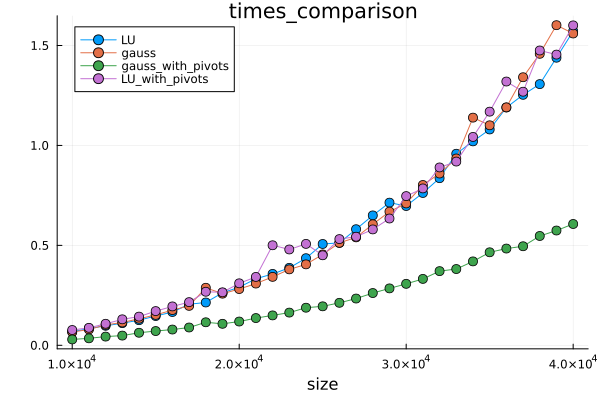
\includegraphics[width=0.6\textwidth]{./graphs/times_comparison.png}
	    \\{Porównanie na podstawie czasu (w sekundach)}
	\end{figure}

\clearpage

	\begin{figure}[h]
	    \centering
	    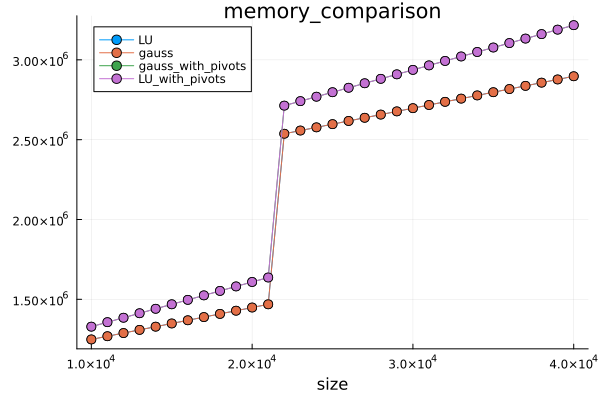
\includegraphics[width=0.6\textwidth]{./graphs/memory_comparison.png}
	    \\{Porównanie na podstawie pamięci (w bajtach)}
	\end{figure}

	Widzimy, że w zakresie pamięci przeprowadzone optymalizacje wykazują wysoką skuteczność. Algorytmy pracujące na modelu macierzy zwykłych potrzebowałyby znacznie więcej zużytej pamięci do wykonania danych obliczeń. Zaobserwowane skoki w ilości zużytych bajtów wynikają prawdopodobnie z wewnętrznego zachowania struktury SparseArrays, która może dynamicznie powiększać swój rozmiar na potrzeby przechowywania większej liczby wartości\\


	Algorytmy z zastosowaniem wyboru elementu głównego na wykresach zobowiązane są do przeprowadzania permutacji rzędów macierzy przed rozpoczęciem obliczeń, co prowadzi do ich niższej wydajności w porównaniu do wariantów bez tego mechanizmu. Natomiast algorytmy LU ustępują naszym modyfikacjom metody Gaussa ze względu na konieczność rzeczywistego wypełnienia dwóch macierzy zamiast jednej, a następnie konieczność rozwiązania obu z nich. To zdecydowanie wpływa na ich efektywność w procesie rozwiązywania układów równań.

\subsection*{Wnioski}
	Prawidłowa analiza problemu może znacząco ułatwić uzyskanie rozwiązania, które w pierwszym, łagodniejszym podejściu wydawało się kosztowne lub wręcz niemożliwe do osiągnięcia. Drobne modyfikacje pierwotnych algorytmów pozwoliły nam istotnie ograniczyć ich złożoność obliczeniową. Posiadając pełną wiedzę na temat struktury danych, zdołaliśmy również zminimalizować zużycie pamięci, starannie dobierając najbardziej ekonomiczny sposób ich przechowywania.


\end{document}